\documentclass[1p]{elsarticle_modified}
%\bibliographystyle{elsarticle-num}

%\usepackage[colorlinks]{hyperref}
%\usepackage{abbrmath_seonhwa} %\Abb, \Ascr, \Acal ,\Abf, \Afrak
\usepackage{amsfonts}
\usepackage{amssymb}
\usepackage{amsmath}
\usepackage{amsthm}
\usepackage{scalefnt}
\usepackage{amsbsy}
\usepackage{kotex}
\usepackage{caption}
\usepackage{subfig}
\usepackage{color}
\usepackage{graphicx}
\usepackage{xcolor} %% white, black, red, green, blue, cyan, magenta, yellow
\usepackage{float}
\usepackage{setspace}
\usepackage{hyperref}

\usepackage{tikz}
\usetikzlibrary{arrows}

\usepackage{multirow}
\usepackage{array} % fixed length table
\usepackage{hhline}

%%%%%%%%%%%%%%%%%%%%%
\makeatletter
\renewcommand*\env@matrix[1][\arraystretch]{%
	\edef\arraystretch{#1}%
	\hskip -\arraycolsep
	\let\@ifnextchar\new@ifnextchar
	\array{*\c@MaxMatrixCols c}}
\makeatother %https://tex.stackexchange.com/questions/14071/how-can-i-increase-the-line-spacing-in-a-matrix
%%%%%%%%%%%%%%%

\usepackage[normalem]{ulem}

\newcommand{\msout}[1]{\ifmmode\text{\sout{\ensuremath{#1}}}\else\sout{#1}\fi}
%SOURCE: \msout is \stkout macro in https://tex.stackexchange.com/questions/20609/strikeout-in-math-mode

\newcommand{\cancel}[1]{
	\ifmmode
	{\color{red}\msout{#1}}
	\else
	{\color{red}\sout{#1}}
	\fi
}

\newcommand{\add}[1]{
	{\color{blue}\uwave{#1}}
}

\newcommand{\replace}[2]{
	\ifmmode
	{\color{red}\msout{#1}}{\color{blue}\uwave{#2}}
	\else
	{\color{red}\sout{#1}}{\color{blue}\uwave{#2}}
	\fi
}

\newcommand{\Sol}{\mathcal{S}} %segment
\newcommand{\D}{D} %diagram
\newcommand{\A}{\mathcal{A}} %arc


%%%%%%%%%%%%%%%%%%%%%%%%%%%%%5 test

\def\sl{\operatorname{\textup{SL}}(2,\Cbb)}
\def\psl{\operatorname{\textup{PSL}}(2,\Cbb)}
\def\quan{\mkern 1mu \triangleright \mkern 1mu}

\theoremstyle{definition}
\newtheorem{thm}{Theorem}[section]
\newtheorem{prop}[thm]{Proposition}
\newtheorem{lem}[thm]{Lemma}
\newtheorem{ques}[thm]{Question}
\newtheorem{cor}[thm]{Corollary}
\newtheorem{defn}[thm]{Definition}
\newtheorem{exam}[thm]{Example}
\newtheorem{rmk}[thm]{Remark}
\newtheorem{alg}[thm]{Algorithm}

\newcommand{\I}{\sqrt{-1}}
\begin{document}

%\begin{frontmatter}
%
%\title{Boundary parabolic representations of knots up to 8 crossings}
%
%%% Group authors per affiliation:
%\author{Yunhi Cho} 
%\address{Department of Mathematics, University of Seoul, Seoul, Korea}
%\ead{yhcho@uos.ac.kr}
%
%
%\author{Seonhwa Kim} %\fnref{s_kim}}
%\address{Center for Geometry and Physics, Institute for Basic Science, Pohang, 37673, Korea}
%\ead{ryeona17@ibs.re.kr}
%
%\author{Hyuk Kim}
%\address{Department of Mathematical Sciences, Seoul National University, Seoul 08826, Korea}
%\ead{hyukkim@snu.ac.kr}
%
%\author{Seokbeom Yoon}
%\address{Department of Mathematical Sciences, Seoul National University, Seoul, 08826,  Korea}
%\ead{sbyoon15@snu.ac.kr}
%
%\begin{abstract}
%We find all boundary parabolic representation of knots up to 8 crossings.
%
%\end{abstract}
%\begin{keyword}
%    \MSC[2010] 57M25 
%\end{keyword}
%
%\end{frontmatter}

%\linenumbers
%\tableofcontents
%
\newcommand\colored[1]{\textcolor{white}{\rule[-0.35ex]{0.8em}{1.4ex}}\kern-0.8em\color{red} #1}%
%\newcommand\colored[1]{\textcolor{white}{ #1}\kern-2.17ex	\textcolor{white}{ #1}\kern-1.81ex	\textcolor{white}{ #1}\kern-2.15ex\color{red}#1	}

{\Large $\underline{12n_{0478}~(K12n_{0478})}$}

\setlength{\tabcolsep}{10pt}
\renewcommand{\arraystretch}{1.6}
\vspace{1cm}\begin{tabular}{m{100pt}>{\centering\arraybackslash}m{274pt}}
\multirow{5}{120pt}{
	\centering
	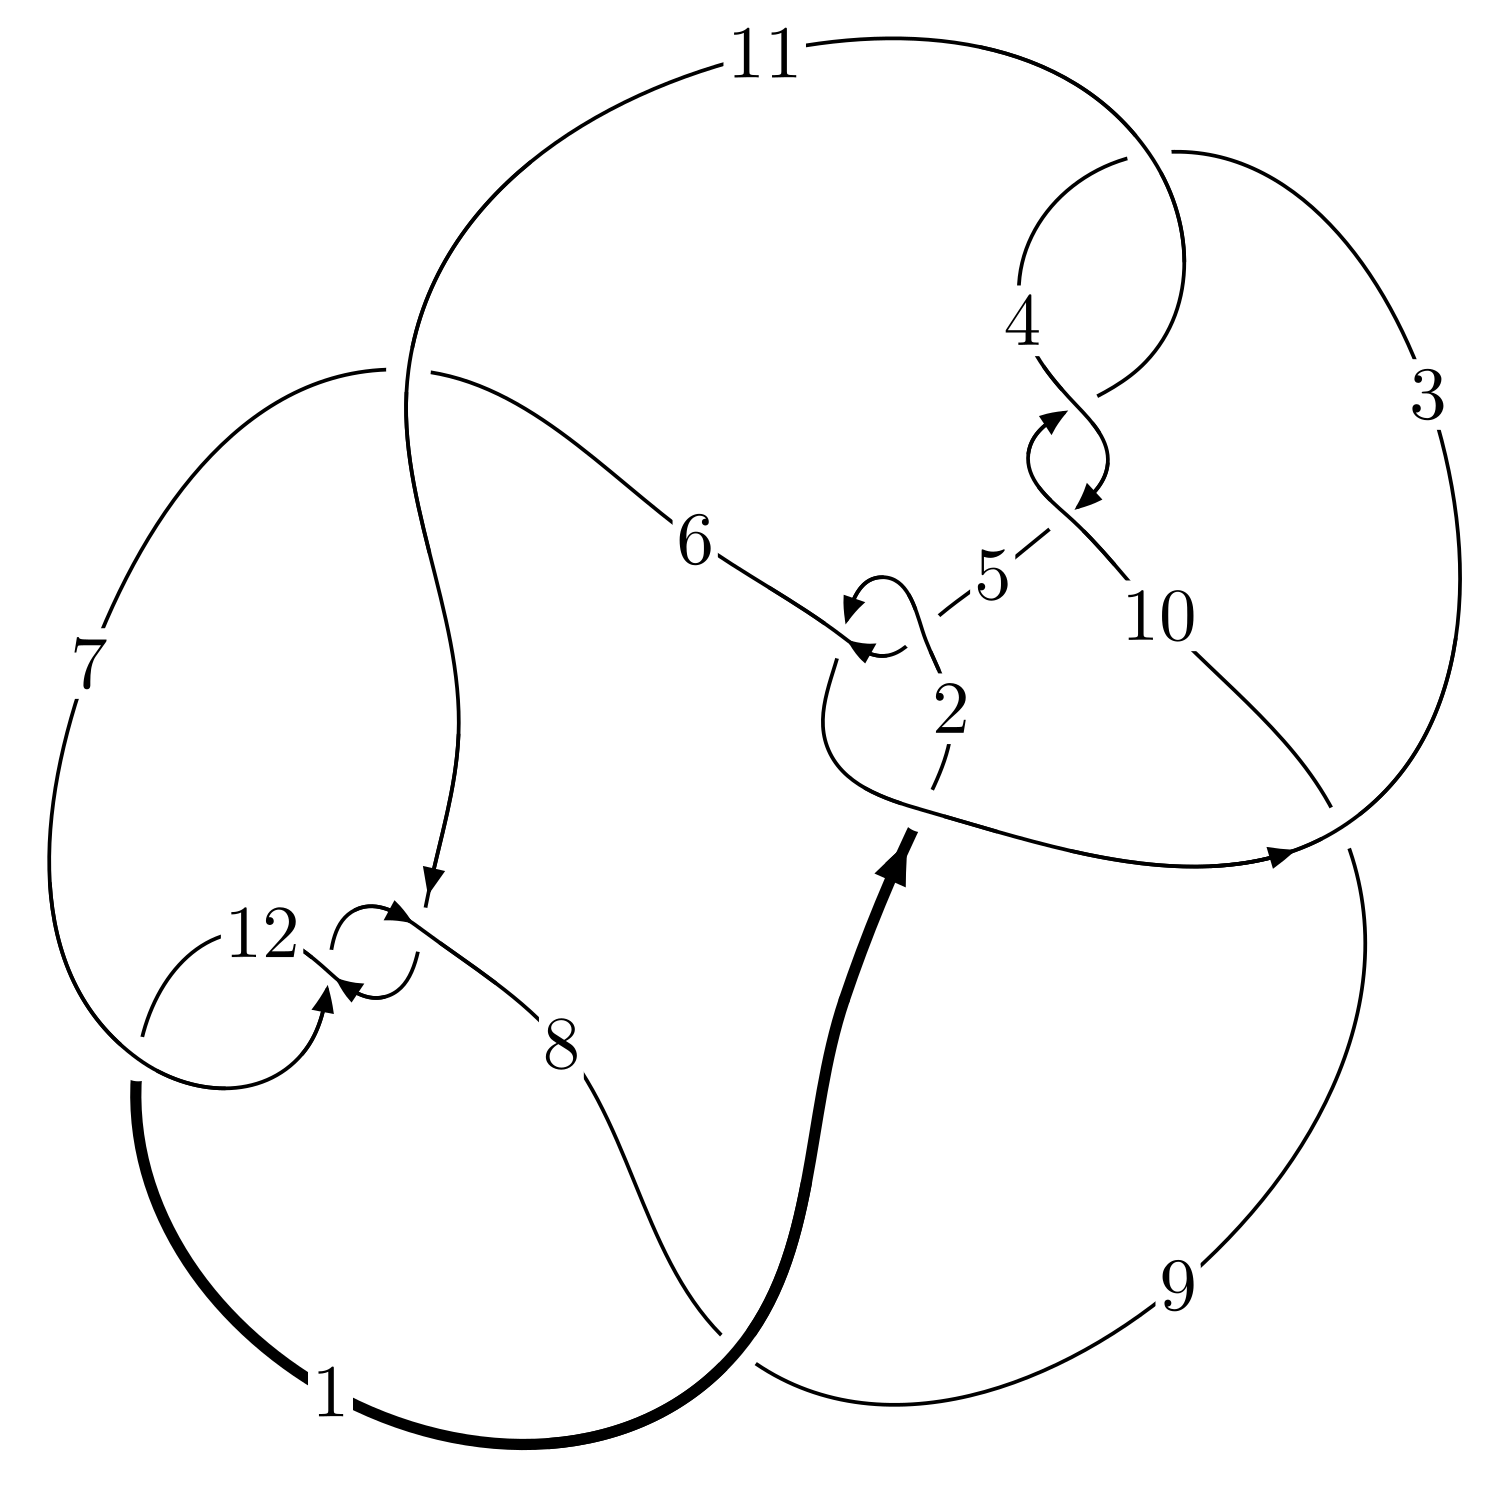
\includegraphics[width=112pt]{../../../GIT/diagram.site/Diagrams/png/2567_12n_0478.png}\\
\ \ \ A knot diagram\footnotemark}&
\allowdisplaybreaks
\textbf{Linearized knot diagam} \\
\cline{2-2}
 &
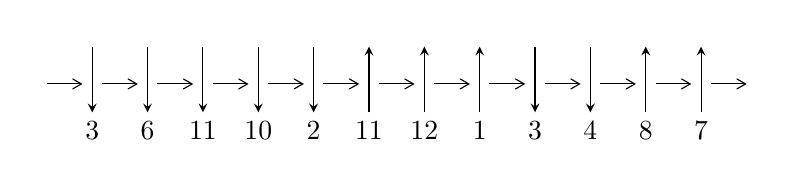
\begin{tikzpicture}[x=20pt, y=17pt]
	% nodes
	\node (C0) at (0, 0) {};
	\node (C1) at (1, 0) {};
	\node (C1U) at (1, +1) {};
	\node (C1D) at (1, -1) {3};

	\node (C2) at (2, 0) {};
	\node (C2U) at (2, +1) {};
	\node (C2D) at (2, -1) {6};

	\node (C3) at (3, 0) {};
	\node (C3U) at (3, +1) {};
	\node (C3D) at (3, -1) {11};

	\node (C4) at (4, 0) {};
	\node (C4U) at (4, +1) {};
	\node (C4D) at (4, -1) {10};

	\node (C5) at (5, 0) {};
	\node (C5U) at (5, +1) {};
	\node (C5D) at (5, -1) {2};

	\node (C6) at (6, 0) {};
	\node (C6U) at (6, +1) {};
	\node (C6D) at (6, -1) {11};

	\node (C7) at (7, 0) {};
	\node (C7U) at (7, +1) {};
	\node (C7D) at (7, -1) {12};

	\node (C8) at (8, 0) {};
	\node (C8U) at (8, +1) {};
	\node (C8D) at (8, -1) {1};

	\node (C9) at (9, 0) {};
	\node (C9U) at (9, +1) {};
	\node (C9D) at (9, -1) {3};

	\node (C10) at (10, 0) {};
	\node (C10U) at (10, +1) {};
	\node (C10D) at (10, -1) {4};

	\node (C11) at (11, 0) {};
	\node (C11U) at (11, +1) {};
	\node (C11D) at (11, -1) {8};

	\node (C12) at (12, 0) {};
	\node (C12U) at (12, +1) {};
	\node (C12D) at (12, -1) {7};
	\node (C13) at (13, 0) {};

	% arrows
	\draw[->,>={angle 60}]
	(C0) edge (C1) (C1) edge (C2) (C2) edge (C3) (C3) edge (C4) (C4) edge (C5) (C5) edge (C6) (C6) edge (C7) (C7) edge (C8) (C8) edge (C9) (C9) edge (C10) (C10) edge (C11) (C11) edge (C12) (C12) edge (C13) ;	\draw[->,>=stealth]
	(C1U) edge (C1D) (C2U) edge (C2D) (C3U) edge (C3D) (C4U) edge (C4D) (C5U) edge (C5D) (C6D) edge (C6U) (C7D) edge (C7U) (C8D) edge (C8U) (C9U) edge (C9D) (C10U) edge (C10D) (C11D) edge (C11U) (C12D) edge (C12U) ;
	\end{tikzpicture} \\
\hhline{~~} \\& 
\textbf{Solving Sequence} \\ \cline{2-2} 
 &
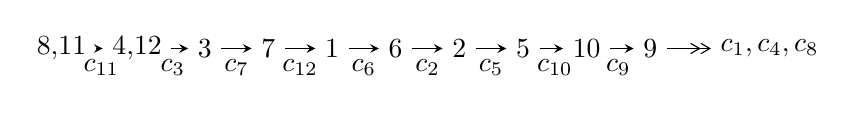
\begin{tikzpicture}[x=23pt, y=7pt]
	% node
	\node (A0) at (-1/8, 0) {8,11};
	\node (A1) at (17/16, 0) {4,12};
	\node (A2) at (17/8, 0) {3};
	\node (A3) at (25/8, 0) {7};
	\node (A4) at (33/8, 0) {1};
	\node (A5) at (41/8, 0) {6};
	\node (A6) at (49/8, 0) {2};
	\node (A7) at (57/8, 0) {5};
	\node (A8) at (65/8, 0) {10};
	\node (A9) at (73/8, 0) {9};
	\node (C1) at (1/2, -1) {$c_{11}$};
	\node (C2) at (13/8, -1) {$c_{3}$};
	\node (C3) at (21/8, -1) {$c_{7}$};
	\node (C4) at (29/8, -1) {$c_{12}$};
	\node (C5) at (37/8, -1) {$c_{6}$};
	\node (C6) at (45/8, -1) {$c_{2}$};
	\node (C7) at (53/8, -1) {$c_{5}$};
	\node (C8) at (61/8, -1) {$c_{10}$};
	\node (C9) at (69/8, -1) {$c_{9}$};
	\node (A10) at (11, 0) {$c_{1},c_{4},c_{8}$};

	% edge
	\draw[->,>=stealth]	
	(A0) edge (A1) (A1) edge (A2) (A2) edge (A3) (A3) edge (A4) (A4) edge (A5) (A5) edge (A6) (A6) edge (A7) (A7) edge (A8) (A8) edge (A9) ;
	\draw[->>,>={angle 60}]	
	(A9) edge (A10);
\end{tikzpicture} \\ 

\end{tabular} \\

\footnotetext{
The image of knot diagram is generated by the software ``\textbf{Draw programme}" developed by Andrew Bartholomew(\url{http://www.layer8.co.uk/maths/draw/index.htm\#Running-draw}), where we modified some parts for our purpose(\url{https://github.com/CATsTAILs/LinksPainter}).
}\phantom \\ \newline 
\centering \textbf{Ideals for irreducible components\footnotemark of $X_{\text{par}}$} 
 
\begin{align*}
I^u_{1}&=\langle 
-271083 u^{22}+222451 u^{21}+\cdots+3670918 b-2822596,\\
\phantom{I^u_{1}}&\phantom{= \langle  }4443679 u^{22}-7680194 u^{21}+\cdots+11012754 a-1652360,\;u^{23}-2 u^{22}+\cdots+u+3\rangle \\
I^u_{2}&=\langle 
b,\;- u^2+a-1,\;u^3- u^2+2 u-1\rangle \\
I^u_{3}&=\langle 
- u^2 a-2 a u-3 u^2+5 b+a- u-2,\;-2 u^2 a+a^2+9 u^2-2 a+7 u+18,\;u^3+u^2+2 u+1\rangle \\
\\
\end{align*}
\raggedright * 3 irreducible components of $\dim_{\mathbb{C}}=0$, with total 32 representations.\\
\footnotetext{All coefficients of polynomials are rational numbers. But the coefficients are sometimes approximated in decimal forms when there is not enough margin.}
\newpage
\renewcommand{\arraystretch}{1}
\centering \section*{I. $I^u_{1}= \langle -2.71\times10^{5} u^{22}+2.22\times10^{5} u^{21}+\cdots+3.67\times10^{6} b-2.82\times10^{6},\;4.44\times10^{6} u^{22}-7.68\times10^{6} u^{21}+\cdots+1.10\times10^{7} a-1.65\times10^{6},\;u^{23}-2 u^{22}+\cdots+u+3 \rangle$}
\flushleft \textbf{(i) Arc colorings}\\
\begin{tabular}{m{7pt} m{180pt} m{7pt} m{180pt} }
\flushright $a_{8}=$&$\begin{pmatrix}0\\u\end{pmatrix}$ \\
\flushright $a_{11}=$&$\begin{pmatrix}1\\0\end{pmatrix}$ \\
\flushright $a_{4}=$&$\begin{pmatrix}-0.403503 u^{22}+0.697391 u^{21}+\cdots-2.67020 u+0.150041\\0.0738461 u^{22}-0.0605982 u^{21}+\cdots-0.383893 u+0.768907\end{pmatrix}$ \\
\flushright $a_{12}=$&$\begin{pmatrix}1\\- u^2\end{pmatrix}$ \\
\flushright $a_{3}=$&$\begin{pmatrix}-0.329657 u^{22}+0.636793 u^{21}+\cdots-3.05409 u+0.918948\\0.0738461 u^{22}-0.0605982 u^{21}+\cdots-0.383893 u+0.768907\end{pmatrix}$ \\
\flushright $a_{7}=$&$\begin{pmatrix}- u\\u^3+u\end{pmatrix}$ \\
\flushright $a_{1}=$&$\begin{pmatrix}u^2+1\\- u^4-2 u^2\end{pmatrix}$ \\
\flushright $a_{6}=$&$\begin{pmatrix}- u^3-2 u\\u^3+u\end{pmatrix}$ \\
\flushright $a_{2}=$&$\begin{pmatrix}-0.366882 u^{22}+0.480327 u^{21}+\cdots-3.32904 u+0.381697\\0.00183360 u^{22}+0.212168 u^{21}+\cdots-0.461364 u+0.884270\end{pmatrix}$ \\
\flushright $a_{5}=$&$\begin{pmatrix}-0.280544 u^{22}+0.210668 u^{21}+\cdots+0.417855 u-1.55795\\0.0945336 u^{22}+0.274635 u^{21}+\cdots+0.828867 u+0.895667\end{pmatrix}$ \\
\flushright $a_{10}=$&$\begin{pmatrix}-0.302116 u^{22}+1.00913 u^{21}+\cdots-1.05470 u+1.52594\\0.382872 u^{22}-0.834070 u^{21}+\cdots+1.92264 u+0.119951\end{pmatrix}$ \\
\flushright $a_{9}=$&$\begin{pmatrix}u^5+2 u^3+u\\- u^7-3 u^5-2 u^3+u\end{pmatrix}$\\&\end{tabular}
\flushleft \textbf{(ii) Obstruction class $= -1$}\\~\\
\flushleft \textbf{(iii) Cusp Shapes $= -\frac{2296634}{1835459} u^{22}+\frac{2776211}{1835459} u^{21}+\cdots+\frac{26517006}{1835459} u-\frac{9454146}{1835459}$}\\~\\
\newpage\renewcommand{\arraystretch}{1}
\flushleft \textbf{(iv) u-Polynomials at the component}\newline \\
\begin{tabular}{m{50pt}|m{274pt}}
Crossings & \hspace{64pt}u-Polynomials at each crossing \\
\hline $$\begin{aligned}c_{1}\end{aligned}$$&$\begin{aligned}
&u^{23}+28 u^{21}+\cdots-166 u+289
\end{aligned}$\\
\hline $$\begin{aligned}c_{2},c_{5}\end{aligned}$$&$\begin{aligned}
&u^{23}+4 u^{22}+\cdots-36 u+17
\end{aligned}$\\
\hline $$\begin{aligned}c_{3},c_{4},c_{10}\end{aligned}$$&$\begin{aligned}
&u^{23}+u^{22}+\cdots+16 u+8
\end{aligned}$\\
\hline $$\begin{aligned}c_{6},c_{8}\end{aligned}$$&$\begin{aligned}
&u^{23}+2 u^{22}+\cdots-11 u+3
\end{aligned}$\\
\hline $$\begin{aligned}c_{7},c_{11},c_{12}\end{aligned}$$&$\begin{aligned}
&u^{23}-2 u^{22}+\cdots+u+3
\end{aligned}$\\
\hline $$\begin{aligned}c_{9}\end{aligned}$$&$\begin{aligned}
&u^{23}- u^{22}+\cdots+41840 u+16424
\end{aligned}$\\
\hline
\end{tabular}\\~\\
\newpage\renewcommand{\arraystretch}{1}
\flushleft \textbf{(v) Riley Polynomials at the component}\newline \\
\begin{tabular}{m{50pt}|m{274pt}}
Crossings & \hspace{64pt}Riley Polynomials at each crossing \\
\hline $$\begin{aligned}c_{1}\end{aligned}$$&$\begin{aligned}
&y^{23}+56 y^{22}+\cdots+17730 y-83521
\end{aligned}$\\
\hline $$\begin{aligned}c_{2},c_{5}\end{aligned}$$&$\begin{aligned}
&y^{23}+28 y^{21}+\cdots-166 y-289
\end{aligned}$\\
\hline $$\begin{aligned}c_{3},c_{4},c_{10}\end{aligned}$$&$\begin{aligned}
&y^{23}+37 y^{22}+\cdots-384 y-64
\end{aligned}$\\
\hline $$\begin{aligned}c_{6},c_{8}\end{aligned}$$&$\begin{aligned}
&y^{23}-38 y^{22}+\cdots+235 y-9
\end{aligned}$\\
\hline $$\begin{aligned}c_{7},c_{11},c_{12}\end{aligned}$$&$\begin{aligned}
&y^{23}+18 y^{22}+\cdots+91 y-9
\end{aligned}$\\
\hline $$\begin{aligned}c_{9}\end{aligned}$$&$\begin{aligned}
&y^{23}+121 y^{22}+\cdots-5779227136 y-269747776
\end{aligned}$\\
\hline
\end{tabular}\\~\\
\newpage\flushleft \textbf{(vi) Complex Volumes and Cusp Shapes}
$$\begin{array}{c|c|c}  
\text{Solutions to }I^u_{1}& \I (\text{vol} + \sqrt{-1}CS) & \text{Cusp shape}\\
 \hline 
\begin{aligned}
u &= \phantom{-}0.264719 + 0.995849 I \\
a &= \phantom{-}0.027236 + 0.839660 I \\
b &= \phantom{-}0.655248 - 0.393424 I\end{aligned}
 & -0.87049 + 1.94619 I & -1.46427 - 4.12692 I \\ \hline\begin{aligned}
u &= \phantom{-}0.264719 - 0.995849 I \\
a &= \phantom{-}0.027236 - 0.839660 I \\
b &= \phantom{-}0.655248 + 0.393424 I\end{aligned}
 & -0.87049 - 1.94619 I & -1.46427 + 4.12692 I \\ \hline\begin{aligned}
u &= \phantom{-}1.044080 + 0.096245 I \\
a &= -0.18594 - 4.05927 I \\
b &= -0.15025 + 1.91664 I\end{aligned}
 & -19.4801 + 4.8275 I & \phantom{-}2.71629 - 2.13422 I \\ \hline\begin{aligned}
u &= \phantom{-}1.044080 - 0.096245 I \\
a &= -0.18594 + 4.05927 I \\
b &= -0.15025 - 1.91664 I\end{aligned}
 & -19.4801 - 4.8275 I & \phantom{-}2.71629 + 2.13422 I \\ \hline\begin{aligned}
u &= -0.120294 + 0.936784 I \\
a &= -1.30367 + 2.24060 I \\
b &= -0.17471 - 1.45617 I\end{aligned}
 & \phantom{-}1.85828 - 0.56096 I & -1.43838 - 0.02221 I \\ \hline\begin{aligned}
u &= -0.120294 - 0.936784 I \\
a &= -1.30367 - 2.24060 I \\
b &= -0.17471 + 1.45617 I\end{aligned}
 & \phantom{-}1.85828 + 0.56096 I & -1.43838 + 0.02221 I \\ \hline\begin{aligned}
u &= -0.869378 + 0.140608 I \\
a &= \phantom{-}0.73050 - 3.00673 I \\
b &= -0.40991 + 1.42355 I\end{aligned}
 & \phantom{-}7.57385 + 1.52871 I & \phantom{-}4.02521 - 0.99137 I \\ \hline\begin{aligned}
u &= -0.869378 - 0.140608 I \\
a &= \phantom{-}0.73050 + 3.00673 I \\
b &= -0.40991 - 1.42355 I\end{aligned}
 & \phantom{-}7.57385 - 1.52871 I & \phantom{-}4.02521 + 0.99137 I \\ \hline\begin{aligned}
u &= -0.149742 + 1.181310 I \\
a &= -0.396431 - 1.221600 I \\
b &= -0.393766 + 0.448599 I\end{aligned}
 & -4.34222 - 1.67723 I & -4.81280 - 1.55068 I \\ \hline\begin{aligned}
u &= -0.149742 - 1.181310 I \\
a &= -0.396431 + 1.221600 I \\
b &= -0.393766 - 0.448599 I\end{aligned}
 & -4.34222 + 1.67723 I & -4.81280 + 1.55068 I\\
 \hline 
 \end{array}$$\newpage$$\begin{array}{c|c|c}  
\text{Solutions to }I^u_{1}& \I (\text{vol} + \sqrt{-1}CS) & \text{Cusp shape}\\
 \hline 
\begin{aligned}
u &= -0.473129 + 1.217800 I \\
a &= \phantom{-}0.56482 - 2.13187 I \\
b &= \phantom{-}0.582006 + 1.271790 I\end{aligned}
 & \phantom{-}4.27129 - 6.38038 I & \phantom{-}0.09560 + 5.13604 I \\ \hline\begin{aligned}
u &= -0.473129 - 1.217800 I \\
a &= \phantom{-}0.56482 + 2.13187 I \\
b &= \phantom{-}0.582006 - 1.271790 I\end{aligned}
 & \phantom{-}4.27129 + 6.38038 I & \phantom{-}0.09560 - 5.13604 I \\ \hline\begin{aligned}
u &= \phantom{-}0.178779 + 1.353110 I \\
a &= -0.400421 - 0.046602 I \\
b &= -0.093563 + 0.525227 I\end{aligned}
 & -4.07440 + 3.45935 I & -1.04248 - 6.69109 I \\ \hline\begin{aligned}
u &= \phantom{-}0.178779 - 1.353110 I \\
a &= -0.400421 + 0.046602 I \\
b &= -0.093563 - 0.525227 I\end{aligned}
 & -4.07440 - 3.45935 I & -1.04248 + 6.69109 I \\ \hline\begin{aligned}
u &= \phantom{-}0.584239 + 1.282930 I \\
a &= -0.96792 - 2.83129 I \\
b &= \phantom{-}0.04217 + 1.93464 I\end{aligned}
 & \phantom{-}16.3629 + 0.9230 I & \phantom{-}0.444071 - 0.918165 I \\ \hline\begin{aligned}
u &= \phantom{-}0.584239 - 1.282930 I \\
a &= -0.96792 + 2.83129 I \\
b &= \phantom{-}0.04217 - 1.93464 I\end{aligned}
 & \phantom{-}16.3629 - 0.9230 I & \phantom{-}0.444071 + 0.918165 I \\ \hline\begin{aligned}
u &= -0.302901 + 1.377090 I \\
a &= -0.93784 + 1.52418 I \\
b &= \phantom{-}0.20153 - 1.48391 I\end{aligned}
 & \phantom{-}2.69974 - 2.64776 I & \phantom{-}0.74921 + 1.92747 I \\ \hline\begin{aligned}
u &= -0.302901 - 1.377090 I \\
a &= -0.93784 - 1.52418 I \\
b &= \phantom{-}0.20153 + 1.48391 I\end{aligned}
 & \phantom{-}2.69974 + 2.64776 I & \phantom{-}0.74921 - 1.92747 I \\ \hline\begin{aligned}
u &= \phantom{-}0.505836 + 0.270726 I \\
a &= \phantom{-}0.610789 + 0.807599 I \\
b &= -0.138145 - 0.624160 I\end{aligned}
 & \phantom{-}0.99412 + 1.06305 I & \phantom{-}3.28669 - 4.14999 I \\ \hline\begin{aligned}
u &= \phantom{-}0.505836 - 0.270726 I \\
a &= \phantom{-}0.610789 - 0.807599 I \\
b &= -0.138145 + 0.624160 I\end{aligned}
 & \phantom{-}0.99412 - 1.06305 I & \phantom{-}3.28669 + 4.14999 I\\
 \hline 
 \end{array}$$\newpage$$\begin{array}{c|c|c}  
\text{Solutions to }I^u_{1}& \I (\text{vol} + \sqrt{-1}CS) & \text{Cusp shape}\\
 \hline 
\begin{aligned}
u &= \phantom{-}0.48292 + 1.39630 I \\
a &= \phantom{-}1.22794 + 2.66452 I \\
b &= \phantom{-}0.21259 - 1.84694 I\end{aligned}
 & \phantom{-}15.3060 + 10.2657 I & -0.43766 - 4.56567 I \\ \hline\begin{aligned}
u &= \phantom{-}0.48292 - 1.39630 I \\
a &= \phantom{-}1.22794 - 2.66452 I \\
b &= \phantom{-}0.21259 + 1.84694 I\end{aligned}
 & \phantom{-}15.3060 - 10.2657 I & -0.43766 + 4.56567 I \\ \hline\begin{aligned}
u &= -0.290242\phantom{ +0.000000I} \\
a &= \phantom{-}1.72852\phantom{ +0.000000I} \\
b &= \phantom{-}0.333618\phantom{ +0.000000I}\end{aligned}
 & -1.11943\phantom{ +0.000000I} & -12.2430\phantom{ +0.000000I}\\
 \hline 
 \end{array}$$\newpage\newpage\renewcommand{\arraystretch}{1}
\centering \section*{II. $I^u_{2}= \langle b,\;- u^2+a-1,\;u^3- u^2+2 u-1 \rangle$}
\flushleft \textbf{(i) Arc colorings}\\
\begin{tabular}{m{7pt} m{180pt} m{7pt} m{180pt} }
\flushright $a_{8}=$&$\begin{pmatrix}0\\u\end{pmatrix}$ \\
\flushright $a_{11}=$&$\begin{pmatrix}1\\0\end{pmatrix}$ \\
\flushright $a_{4}=$&$\begin{pmatrix}u^2+1\\0\end{pmatrix}$ \\
\flushright $a_{12}=$&$\begin{pmatrix}1\\- u^2\end{pmatrix}$ \\
\flushright $a_{3}=$&$\begin{pmatrix}u^2+1\\0\end{pmatrix}$ \\
\flushright $a_{7}=$&$\begin{pmatrix}- u\\u^2- u+1\end{pmatrix}$ \\
\flushright $a_{1}=$&$\begin{pmatrix}u^2+1\\- u^2+u-1\end{pmatrix}$ \\
\flushright $a_{6}=$&$\begin{pmatrix}- u^2-1\\u^2- u+1\end{pmatrix}$ \\
\flushright $a_{2}=$&$\begin{pmatrix}2 u^2+2\\- u^2+u-1\end{pmatrix}$ \\
\flushright $a_{5}=$&$\begin{pmatrix}u^2+1\\0\end{pmatrix}$ \\
\flushright $a_{10}=$&$\begin{pmatrix}1\\0\end{pmatrix}$ \\
\flushright $a_{9}=$&$\begin{pmatrix}1\\0\end{pmatrix}$\\&\end{tabular}
\flushleft \textbf{(ii) Obstruction class $= 1$}\\~\\
\flushleft \textbf{(iii) Cusp Shapes $= 6 u^2-4 u+4$}\\~\\
\newpage\renewcommand{\arraystretch}{1}
\flushleft \textbf{(iv) u-Polynomials at the component}\newline \\
\begin{tabular}{m{50pt}|m{274pt}}
Crossings & \hspace{64pt}u-Polynomials at each crossing \\
\hline $$\begin{aligned}c_{1},c_{2}\end{aligned}$$&$\begin{aligned}
&(u-1)^3
\end{aligned}$\\
\hline $$\begin{aligned}c_{3},c_{4},c_{9}\\c_{10}\end{aligned}$$&$\begin{aligned}
&u^3
\end{aligned}$\\
\hline $$\begin{aligned}c_{5}\end{aligned}$$&$\begin{aligned}
&(u+1)^3
\end{aligned}$\\
\hline $$\begin{aligned}c_{6},c_{8}\end{aligned}$$&$\begin{aligned}
&u^3- u^2+1
\end{aligned}$\\
\hline $$\begin{aligned}c_{7}\end{aligned}$$&$\begin{aligned}
&u^3+u^2+2 u+1
\end{aligned}$\\
\hline $$\begin{aligned}c_{11},c_{12}\end{aligned}$$&$\begin{aligned}
&u^3- u^2+2 u-1
\end{aligned}$\\
\hline
\end{tabular}\\~\\
\newpage\renewcommand{\arraystretch}{1}
\flushleft \textbf{(v) Riley Polynomials at the component}\newline \\
\begin{tabular}{m{50pt}|m{274pt}}
Crossings & \hspace{64pt}Riley Polynomials at each crossing \\
\hline $$\begin{aligned}c_{1},c_{2},c_{5}\end{aligned}$$&$\begin{aligned}
&(y-1)^3
\end{aligned}$\\
\hline $$\begin{aligned}c_{3},c_{4},c_{9}\\c_{10}\end{aligned}$$&$\begin{aligned}
&y^3
\end{aligned}$\\
\hline $$\begin{aligned}c_{6},c_{8}\end{aligned}$$&$\begin{aligned}
&y^3- y^2+2 y-1
\end{aligned}$\\
\hline $$\begin{aligned}c_{7},c_{11},c_{12}\end{aligned}$$&$\begin{aligned}
&y^3+3 y^2+2 y-1
\end{aligned}$\\
\hline
\end{tabular}\\~\\
\newpage\flushleft \textbf{(vi) Complex Volumes and Cusp Shapes}
$$\begin{array}{c|c|c}  
\text{Solutions to }I^u_{2}& \I (\text{vol} + \sqrt{-1}CS) & \text{Cusp shape}\\
 \hline 
\begin{aligned}
u &= \phantom{-}0.215080 + 1.307140 I \\
a &= -0.662359 + 0.562280 I \\
b &= \phantom{-0.000000 } 0\end{aligned}
 & -4.66906 + 2.82812 I & -6.83447 - 1.85489 I \\ \hline\begin{aligned}
u &= \phantom{-}0.215080 - 1.307140 I \\
a &= -0.662359 - 0.562280 I \\
b &= \phantom{-0.000000 } 0\end{aligned}
 & -4.66906 - 2.82812 I & -6.83447 + 1.85489 I \\ \hline\begin{aligned}
u &= \phantom{-}0.569840\phantom{ +0.000000I} \\
a &= \phantom{-}1.32472\phantom{ +0.000000I} \\
b &= \phantom{-0.000000 } 0\end{aligned}
 & -0.531480\phantom{ +0.000000I} & \phantom{-}3.66890\phantom{ +0.000000I}\\
 \hline 
 \end{array}$$\newpage\newpage\renewcommand{\arraystretch}{1}
\centering \section*{III. $I^u_{3}= \langle - u^2 a-2 a u-3 u^2+5 b+a- u-2,\;-2 u^2 a+a^2+9 u^2-2 a+7 u+18,\;u^3+u^2+2 u+1 \rangle$}
\flushleft \textbf{(i) Arc colorings}\\
\begin{tabular}{m{7pt} m{180pt} m{7pt} m{180pt} }
\flushright $a_{8}=$&$\begin{pmatrix}0\\u\end{pmatrix}$ \\
\flushright $a_{11}=$&$\begin{pmatrix}1\\0\end{pmatrix}$ \\
\flushright $a_{4}=$&$\begin{pmatrix}a\\\frac{1}{5} u^2 a+\frac{3}{5} u^2+\cdots-\frac{1}{5} a+\frac{2}{5}\end{pmatrix}$ \\
\flushright $a_{12}=$&$\begin{pmatrix}1\\- u^2\end{pmatrix}$ \\
\flushright $a_{3}=$&$\begin{pmatrix}\frac{1}{5} u^2 a+\frac{3}{5} u^2+\cdots+\frac{4}{5} a+\frac{2}{5}\\\frac{1}{5} u^2 a+\frac{3}{5} u^2+\cdots-\frac{1}{5} a+\frac{2}{5}\end{pmatrix}$ \\
\flushright $a_{7}=$&$\begin{pmatrix}- u\\- u^2- u-1\end{pmatrix}$ \\
\flushright $a_{1}=$&$\begin{pmatrix}u^2+1\\- u^2- u-1\end{pmatrix}$ \\
\flushright $a_{6}=$&$\begin{pmatrix}u^2+1\\- u^2- u-1\end{pmatrix}$ \\
\flushright $a_{2}=$&$\begin{pmatrix}\frac{1}{5} u^2 a+\frac{8}{5} u^2+\cdots+\frac{4}{5} a+\frac{7}{5}\\\frac{1}{5} u^2 a-\frac{2}{5} u^2+\cdots-\frac{1}{5} a-\frac{3}{5}\end{pmatrix}$ \\
\flushright $a_{5}=$&$\begin{pmatrix}-\frac{1}{5} u^2 a-\frac{3}{5} u^2+\cdots-\frac{4}{5} a-\frac{2}{5}\\-\frac{1}{5} u^2 a-\frac{3}{5} u^2+\cdots+\frac{1}{5} a-\frac{2}{5}\end{pmatrix}$ \\
\flushright $a_{10}=$&$\begin{pmatrix}\frac{3}{5} u^2 a-\frac{11}{5} u^2+\cdots+\frac{2}{5} a-\frac{29}{5}\\2\end{pmatrix}$ \\
\flushright $a_{9}=$&$\begin{pmatrix}-1\\0\end{pmatrix}$\\&\end{tabular}
\flushleft \textbf{(ii) Obstruction class $= 1$}\\~\\
\flushleft \textbf{(iii) Cusp Shapes $= 4 u^2+4 u+4$}\\~\\
\newpage\renewcommand{\arraystretch}{1}
\flushleft \textbf{(iv) u-Polynomials at the component}\newline \\
\begin{tabular}{m{50pt}|m{274pt}}
Crossings & \hspace{64pt}u-Polynomials at each crossing \\
\hline $$\begin{aligned}c_{1},c_{5}\end{aligned}$$&$\begin{aligned}
&(u-1)^6
\end{aligned}$\\
\hline $$\begin{aligned}c_{2}\end{aligned}$$&$\begin{aligned}
&(u+1)^6
\end{aligned}$\\
\hline $$\begin{aligned}c_{3},c_{4},c_{9}\\c_{10}\end{aligned}$$&$\begin{aligned}
&(u^2+2)^3
\end{aligned}$\\
\hline $$\begin{aligned}c_{6},c_{8}\end{aligned}$$&$\begin{aligned}
&(u^3+u^2-1)^2
\end{aligned}$\\
\hline $$\begin{aligned}c_{7}\end{aligned}$$&$\begin{aligned}
&(u^3- u^2+2 u-1)^2
\end{aligned}$\\
\hline $$\begin{aligned}c_{11},c_{12}\end{aligned}$$&$\begin{aligned}
&(u^3+u^2+2 u+1)^2
\end{aligned}$\\
\hline
\end{tabular}\\~\\
\newpage\renewcommand{\arraystretch}{1}
\flushleft \textbf{(v) Riley Polynomials at the component}\newline \\
\begin{tabular}{m{50pt}|m{274pt}}
Crossings & \hspace{64pt}Riley Polynomials at each crossing \\
\hline $$\begin{aligned}c_{1},c_{2},c_{5}\end{aligned}$$&$\begin{aligned}
&(y-1)^6
\end{aligned}$\\
\hline $$\begin{aligned}c_{3},c_{4},c_{9}\\c_{10}\end{aligned}$$&$\begin{aligned}
&(y+2)^6
\end{aligned}$\\
\hline $$\begin{aligned}c_{6},c_{8}\end{aligned}$$&$\begin{aligned}
&(y^3- y^2+2 y-1)^2
\end{aligned}$\\
\hline $$\begin{aligned}c_{7},c_{11},c_{12}\end{aligned}$$&$\begin{aligned}
&(y^3+3 y^2+2 y-1)^2
\end{aligned}$\\
\hline
\end{tabular}\\~\\
\newpage\flushleft \textbf{(vi) Complex Volumes and Cusp Shapes}
$$\begin{array}{c|c|c}  
\text{Solutions to }I^u_{3}& \I (\text{vol} + \sqrt{-1}CS) & \text{Cusp shape}\\
 \hline 
\begin{aligned}
u &= -0.215080 + 1.307140 I \\
a &= -1.71575 + 1.02526 I \\
b &= \phantom{-0.000000 } -1.414210 I\end{aligned}
 & \phantom{-}0.26574 - 2.82812 I & -3.50976 + 2.97945 I \\ \hline\begin{aligned}
u &= -0.215080 + 1.307140 I \\
a &= \phantom{-}0.39103 - 2.14982 I \\
b &= \phantom{-0.000000 -}1.414210 I\end{aligned}
 & \phantom{-}0.26574 - 2.82812 I & -3.50976 + 2.97945 I \\ \hline\begin{aligned}
u &= -0.215080 - 1.307140 I \\
a &= -1.71575 - 1.02526 I \\
b &= \phantom{-0.000000 -}1.414210 I\end{aligned}
 & \phantom{-}0.26574 + 2.82812 I & -3.50976 - 2.97945 I \\ \hline\begin{aligned}
u &= -0.215080 - 1.307140 I \\
a &= \phantom{-}0.39103 + 2.14982 I \\
b &= \phantom{-0.000000 } -1.414210 I\end{aligned}
 & \phantom{-}0.26574 + 2.82812 I & -3.50976 - 2.97945 I \\ \hline\begin{aligned}
u &= -0.569840\phantom{ +0.000000I} \\
a &= \phantom{-}1.32472 + 3.89599 I \\
b &= \phantom{-0.000000 } -1.414210 I\end{aligned}
 & \phantom{-}4.40332\phantom{ +0.000000I} & \phantom{-}3.01950\phantom{ +0.000000I} \\ \hline\begin{aligned}
u &= -0.569840\phantom{ +0.000000I} \\
a &= \phantom{-}1.32472 - 3.89599 I \\
b &= \phantom{-0.000000 -}1.414210 I\end{aligned}
 & \phantom{-}4.40332\phantom{ +0.000000I} & \phantom{-}3.01950\phantom{ +0.000000I}\\
 \hline 
 \end{array}$$\newpage
\newpage\renewcommand{\arraystretch}{1}
\centering \section*{ IV. u-Polynomials}
\begin{tabular}{m{50pt}|m{274pt}}
Crossings & \hspace{64pt}u-Polynomials at each crossing \\
\hline $$\begin{aligned}c_{1}\end{aligned}$$&$\begin{aligned}
&((u-1)^9)(u^{23}+28 u^{21}+\cdots-166 u+289)
\end{aligned}$\\
\hline $$\begin{aligned}c_{2}\end{aligned}$$&$\begin{aligned}
&((u-1)^3)(u+1)^6(u^{23}+4 u^{22}+\cdots-36 u+17)
\end{aligned}$\\
\hline $$\begin{aligned}c_{3},c_{4},c_{10}\end{aligned}$$&$\begin{aligned}
&u^3(u^2+2)^3(u^{23}+u^{22}+\cdots+16 u+8)
\end{aligned}$\\
\hline $$\begin{aligned}c_{5}\end{aligned}$$&$\begin{aligned}
&((u-1)^6)(u+1)^3(u^{23}+4 u^{22}+\cdots-36 u+17)
\end{aligned}$\\
\hline $$\begin{aligned}c_{6},c_{8}\end{aligned}$$&$\begin{aligned}
&(u^3- u^2+1)(u^3+u^2-1)^2(u^{23}+2 u^{22}+\cdots-11 u+3)
\end{aligned}$\\
\hline $$\begin{aligned}c_{7}\end{aligned}$$&$\begin{aligned}
&((u^3- u^2+2 u-1)^2)(u^3+u^2+2 u+1)(u^{23}-2 u^{22}+\cdots+u+3)
\end{aligned}$\\
\hline $$\begin{aligned}c_{9}\end{aligned}$$&$\begin{aligned}
&u^3(u^2+2)^3(u^{23}-u^{22}+\cdots+41840 u+16424)
\end{aligned}$\\
\hline $$\begin{aligned}c_{11},c_{12}\end{aligned}$$&$\begin{aligned}
&(u^3- u^2+2 u-1)(u^3+u^2+2 u+1)^2(u^{23}-2 u^{22}+\cdots+u+3)
\end{aligned}$\\
\hline
\end{tabular}\newpage\renewcommand{\arraystretch}{1}
\centering \section*{ V. Riley Polynomials}
\begin{tabular}{m{50pt}|m{274pt}}
Crossings & \hspace{64pt}Riley Polynomials at each crossing \\
\hline $$\begin{aligned}c_{1}\end{aligned}$$&$\begin{aligned}
&((y-1)^9)(y^{23}+56 y^{22}+\cdots+17730 y-83521)
\end{aligned}$\\
\hline $$\begin{aligned}c_{2},c_{5}\end{aligned}$$&$\begin{aligned}
&((y-1)^9)(y^{23}+28 y^{21}+\cdots-166 y-289)
\end{aligned}$\\
\hline $$\begin{aligned}c_{3},c_{4},c_{10}\end{aligned}$$&$\begin{aligned}
&y^3(y+2)^6(y^{23}+37 y^{22}+\cdots-384 y-64)
\end{aligned}$\\
\hline $$\begin{aligned}c_{6},c_{8}\end{aligned}$$&$\begin{aligned}
&((y^3- y^2+2 y-1)^3)(y^{23}-38 y^{22}+\cdots+235 y-9)
\end{aligned}$\\
\hline $$\begin{aligned}c_{7},c_{11},c_{12}\end{aligned}$$&$\begin{aligned}
&((y^3+3 y^2+2 y-1)^3)(y^{23}+18 y^{22}+\cdots+91 y-9)
\end{aligned}$\\
\hline $$\begin{aligned}c_{9}\end{aligned}$$&$\begin{aligned}
&y^3(y+2)^6(y^{23}+121 y^{22}+\cdots-5.77923\times10^{9} y-2.69748\times10^{8})
\end{aligned}$\\
\hline
\end{tabular}
\vskip 2pc
\end{document}